\documentclass[twocolumn]{emulateapj}
\usepackage{graphicx}
\usepackage{hyperref}
\usepackage{float}
\usepackage{multirow}
\usepackage{siunitx}

\shorttitle{Modal Noise Minimization}
\shortauthors{Petersburg et al.}

\begin{document}

\title{Modal Noise Mitigation through Fiber Agitation for Fiber-fed Radial Velocity Spectrographs}

\author{Ryan Petersburg}
\affil{Department of Physics, Yale University}

\author{Tyler McCracken}
\affil{Department of Astronomy, Yale University}

\author{Dominic Eggerman}
\affil{Yale University}

\author{Debra Fischer}
\affil{Department of Astronomy, Yale University}


\begin{abstract}

Optical fiber modal noise is a critically limiting factor to signal-to-noise for high precision spectroscopy in the near-infrared and visible. Unabated, especially for highly coherent light sources, modal noise can induce radial velocity errors that hinder the discovery of low-mass (and potentially earth-like) planets. Previous research in this field has found sufficient modal noise mitigation through use of an integrating sphere, but this requires extremely bright light sources, a luxury not necessarily afforded calibration for the next generation of high resolution optical-range spectrographs. Otherwise, mechanical agitation, which ``mixes'' the fiber's modal patterns and allows the noise to be averaged over minutes-long exposures, provides some noise reduction but the methods have not been fully optimized by the community. Therefore, we have filled out the parameter space of modal noise agitation techniques in order to better understand agitation's contribution to mitigating modal noise and to discover the optimal strategy for agitating fibers. We found that modal noise was best suppressed by the chaotic nature of coupled harmonic motion at high amplitude for fibers with large core diameters and low azimuthal symmetry, reducing modal noise induced radial velocity error to below 10 cm/s. This work has subsequently influenced the design of a fiber agitator to be installed with the Extreme Precision Spectrograph (EXPRES).

\end{abstract}


\section{Introduction}
\label{sec:intro}

Radial velocity (RV) exoplanet detection has continually been on the path of discovering less massive planets. The current goal of RV spectroscopy is \SI{10}{\centi\meter\per\second} precision, thereby allowing the discovery of earth-like planets orbiting sun-like stars in their respective habitable zone \citep{Fischer2016}. Therefore, the next-generation of RV spectrographs require precision engineering and extreme stability to yield such results.

Multimode fibers have thus become the backbone of RV spectrograph design. Light from the slewing telescope focus is coupled through a long fiber in order to reach the spectrograph, allowing for greater vibrational and thermal isolation. Also, light from various calibration sources (e.g. laser frequency combs, thorium-argon cells, and flat fielding sources) must be simultaneously coupled into the spectrograph. To reduce the detrimental effects of poor fiber scrambling \citep{Hunter1992, Halverson2015a}, multimode fiber architectures for RV spectrographs now include non-circular fibers with octagonal, rectangular, and square core cross-sections.

In this paper, we attempt to discern the optimal strategy for reducing modal noise, an inherent property of multimode fibers, through mechanical agitation. We begin by defining modal noise and exploring how previous experiments have mitigated it through static and dynamic methods such as fiber agitation (section \ref{sec:modal_noise_intro}. We then describe our own methods of fiber agitation (section \ref{sec:fiber_agitation}) and discuss results from using these methods on fibers of varying cross-sectional shape and coupling permutations (section \ref{sec:results}. Finally, we relate these results to limits in RV precision (section \ref{sec:rv_precision}) and discuss how these results should be applied to next-generation RV spectrographs (section \ref{sec:conclusions}). The work in this paper was conducted to influence design decisions for the Extreme Precision Spectrograph \citep{Jurgenson2016}.

\section{Optical Fiber Modal Noise}
\label{sec:modal_noise_intro}

All multimode step-index optical fibers produce a high-contrast speckle pattern, known as \textit{modal noise}, when propagating light from a highly coherent light source (see figure \ref{fig:fiber_example}). Modal noise is an inherent property of all fibers regardless of the cross-sectional core shape \citep{Sablowski2015} [OTHER CITATIONS?] as long as the core is large enough to propagate multiple electromagnetic modes at a given wavelength. Due to its high contrast, modal noise can severely decrease the signal-to-noise ratio (SNR) of an RV spectrograph \citep{Epworth1978, Baudrand2001, Lemke2011}. Additionally, if the speckle pattern drifts between exposures, especially with some period of motion, modal noise can cause errant RV signatures in the data that is distinct from errors due to poor scrambling \citep{Mahadevan2014}.

\begin{figure}
\centering
	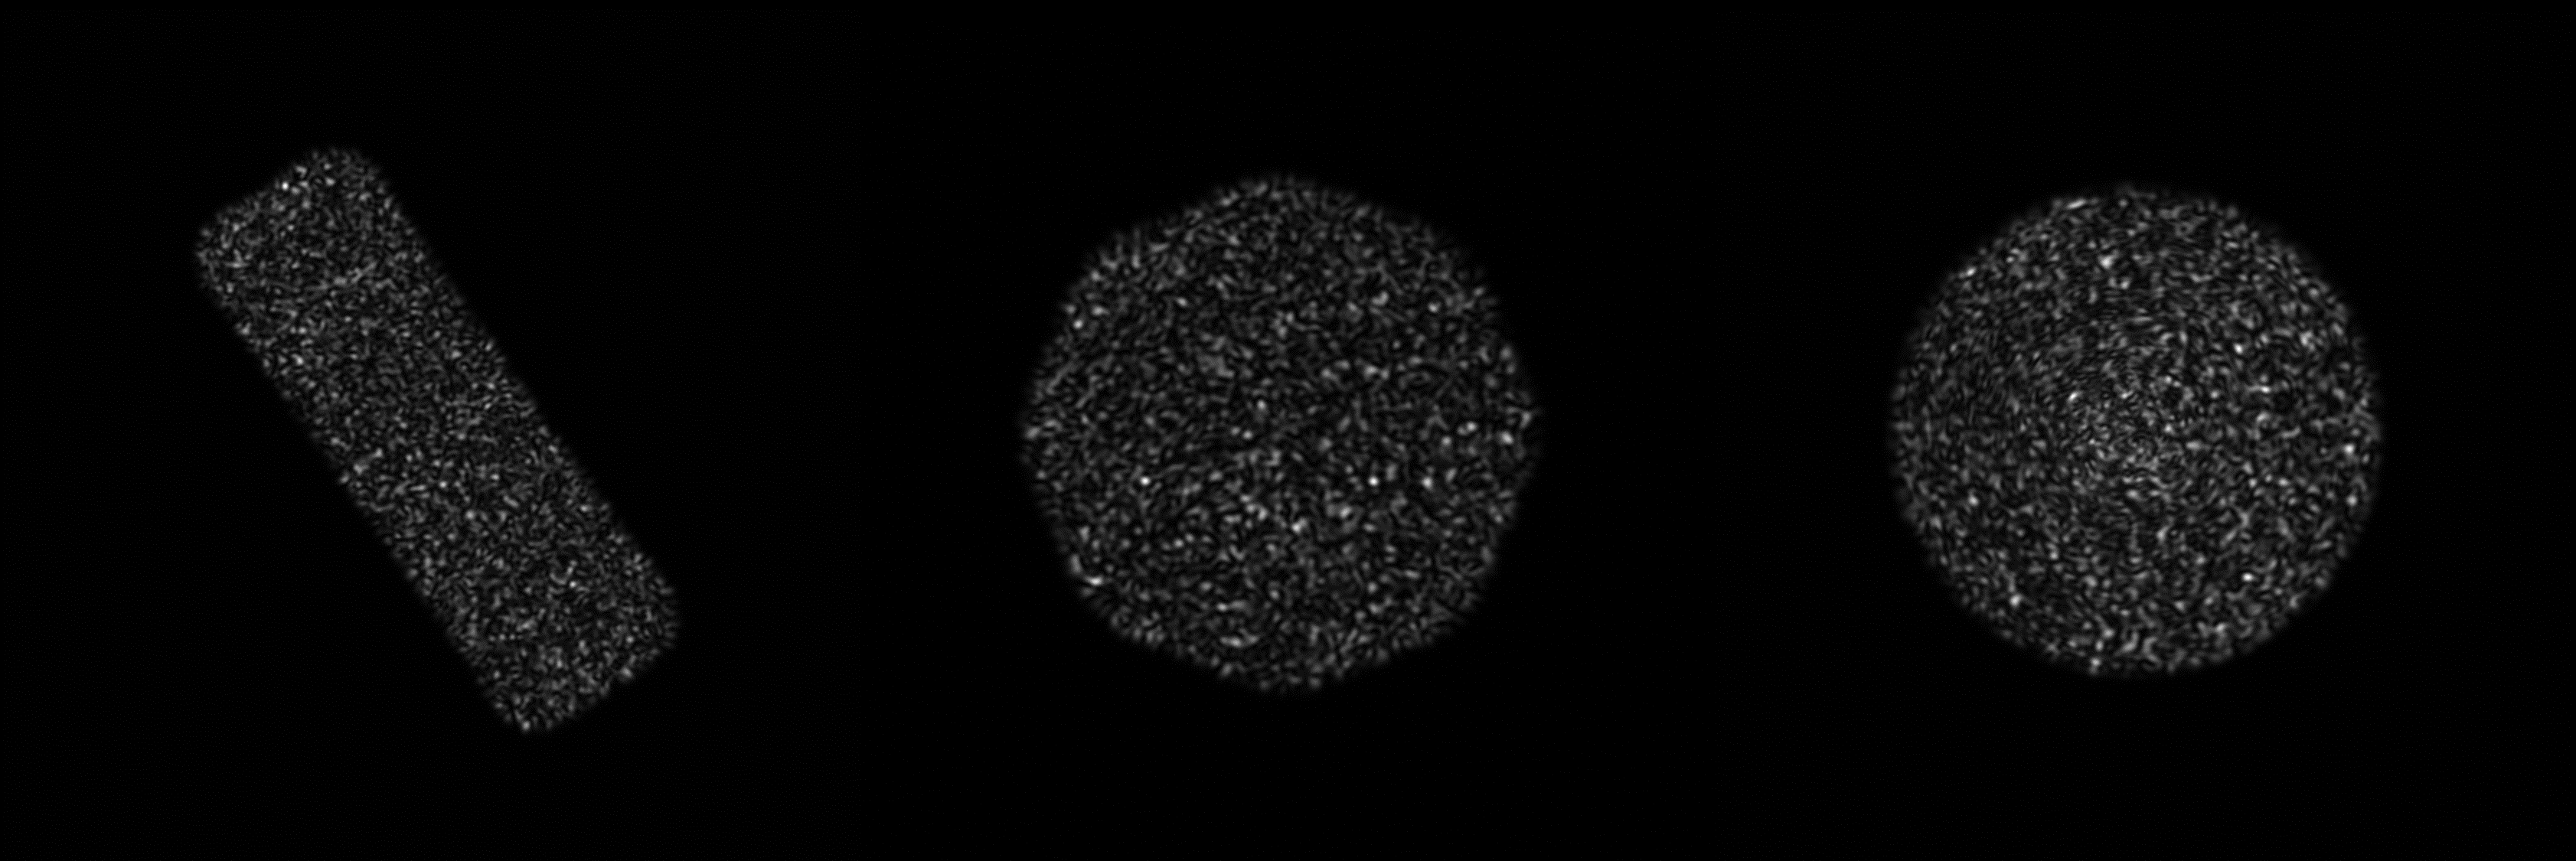
\includegraphics[width=\columnwidth]{images/fiber_example.png}
	\caption{Examples of unmitigated modal noise for a rectangular (left), octagonal (middle), and circular (right) optical fiber. All three fibers shown here have approximately the same cross-sectional area, meaning that they each are propagating about the same number of electromagnetic modes (see section \ref{sec:fiber_agitation}).}
\label{fig:fiber_example}
\end{figure}

Modal noise's dependence on static optical properties has been well documented. Modal noise SNR is increased for larger fiber core diameters \citep{Sablowski2015} [CITE OTHERS HERE] and for non-circular fibers over circular fibers \citep{Sturmer2016, Sablowski2015} [CITE OTHERS HERE]. Increasing the number of static bends in a fiber slightly increases SNR \citep{Imai1979}. Far field modal noise SNR is strongly anti-correlated with injected focal ratio \citep{Sablowski2015}, while the near field modal noise SNR is independent of injected focal ratio \citep{Baudrand2001}. Finally, modal noise SNR was shown to be anti-correlated with wavelength (for reasons to be discussed in section \ref{sec:fiber_agitation}), poorly responsive to input pupil obstructions, and independent of fiber length \citep{Baudrand2001}.

Modal noise is also affected by dynamic optical properties, meaning it can induce false RV's on the spectrograph, in addition to being an issue of SNR. The speckle pattern imaged at the end of a fiber shifts over time due to many reasons, but most commonly because of \citep{Epworth1978}:
\begin{enumerate}
\item Wavelength drift
\item Temperature variation
\item Fiber input illumination variation
\item Fiber movement (bending, twisting, etc.)
\end{enumerate}
Assuming no wavelength drift due to use of a highly stable wavelength calibration source, the latter three conditions still inevitably pose problems when imaging the spectrum since they are inherent to modern fiber-fed RV spectrographs \citep{Baudrand2001, Mahadevan2014}. It is important to note here that \cite{Epworth1978} also includes spatial filtering as a requirement for complications from modal noise. Spatial filtering is historically assumed since many RV experiments use rectangular slits over circular fibers when injecting light into the spectrograph optics. However, as shown in section \ref{sec:rv_precision}, modal noise is still a detriment to RV precision even for an unfiltered rectangular fiber, therefore the spatial filter requirement has been removed.

The resultant RV shift ($\Delta RV$) due to a shifting speckle pattern centroid at the end of a fiber is calculated in a similar manner to scrambling gain [CITATION]:
\begin{equation}
\Delta RV = \frac{c}{R} \frac{\Delta d}{D}
\label{eq:rv_error}
\end{equation}
where $c$ is the speed of light in a vacuum, $R$ is the resolution of the spectrograph, $\Delta d$ is the shift in the centroid of the fiber in the dispersion direction and $D$ is the diameter of the fiber (or slit) in the dispersion direction. Notice that for a $R=150,000$ spectrograph fed by a \SI{33}{\micro\meter} slit attempting to reach \SI{1}{\meter\per\second} RV precision per wavelength calibration line, the required stability of the centroid along the dispersion direction is \SI{0.165}{\micro\meter}.

Modal noise can be reduced for a coherent light source by continuously exacerbating one of the above four causes of drift, thereby shifting the speckle pattern during an appropriately long integration time and subsequently averaging out the noise. Option 1 is not feasible due to the wavelength sensitivity of an RV spectrograph. Controlled temperature variation is difficult because a 1 meter fiber requires approximately $8 ^\circ \textrm{C}$ fluctuations to visibly decorrelate the speckle pattern \citep{Redding2013} [MORE CITATIONS???] and the spectrograph environment should remain thermally stable for higher precision [CITATION???]. Therefore, RV spectrographs have been left with either varying the illumination (option 3) or shaking the fiber (option 4).

First, we would like to note that some RV spectrographs [CITATIONS NEEDED, e.g. iLocator] have moved to a completely single mode fiber architecture to help alleviate the complications of modal noise without agitation or illumination variation. However, single-mode fibers have a very limited bandwidth over which they propagate a single-mode, meaning they may not be truly single-mode for broadband wavelength calibration. Also, \cite{Halverson2015b} asserts that a type of ``modal noise'' due to polarization may also exist in single mode fibers. Thus, the study of modal noise reduction methods may still be necessary even for these novel single-mode-fiber injected instruments.

\begin{table*}
\centering
\caption{Previous study of dynamic modal noise mitigation methods}
	\begin{tabular}{cccc}
		\hline
		Reference & Method & Frequency & Amplitude \\
		\hline\hline
		\cite{Daino1980} & Loudspeaker & 110 Hz & ``Sufficient'' \\
		\hline
		\cite{Baudrand2001} & --- & 30 Hz & 1 mm \\
		\hline
		\multirow{2}{*}{\cite{Lemke2011}} & Loudspeaker & 1.5 Hz & --- \\
		 & Loudspeaker & 80 Hz & --- \\
		\hline
		\multirow{3}{*}{\cite{McCoy2012}} & Paint mixer & 60 Hz & --- \\
		 & Hand agitated & 1-2 Hz & 10-15 cm \\
		 & Mechanical agitator & ``Low'' & ``High''\\
		\hline
		\multirow{2}{*}{\cite{Plavchan2013}} & ``Tweeter'' & 100 Hz & 1 mm \\
		 & ``Woofer'' & 1 Hz & 25 mm \\
		\hline
		\multirow{3}{*}{\cite{Mahadevan2014}} & Int. Sph. + Diff. & --- & ---\\
		 & McCoy agitator & ``Low'' & ``High' \\
		 & Hand agitation & 1-2 Hz & 10 cm \\
		\hline
		\multirow{2}{*}{\cite{Halverson2014}} & Int. Sph. + Diff. & --- & --- \\
		 & Int. Sph. + OAP & --- & --- \\
		\hline		
		\cite{Roy2014} & Rail agitator & ``Low'' & ``High'' \\
		\hline
		\cite{Sablowski2015} & Mechanical ``Excenter''& 2 Hz & 20 cm \\
		\hline
	\end{tabular}
\label{table:previous_studies}
\end{table*}

As summarized in table \ref{table:previous_studies}, modal noise reduction techniques have been discussed by many experiments concerned with RV spectroscopy. \cite{Mahadevan2014} and \cite{Halverson2014} have shown the effectiveness of illumination variation using an integrating sphere, diffuser, and rotating off-axis parabolic mirror. These studies presented the gradual improvements in modal noise reduction due to the addition of further illumination variation. They also showed how these techniques would reliably reduce modal noise RV error to an upper limit of 1.3 m/s per line, leading to a total RV precision of 20-30 cm/s for an $R = 50,000$ instrument. However, the integrating sphere, an integral part of these methods, has a throughput efficiency of approximately $10^{-6}$. Therefore, this result is promising for extremely bright calibration sources that are available in the near infrared, but may not be useful for ultra-precise optical laser frequency combs which contain about [POWER VALUE AND PHOTON COUNT NEEDED] for each comb line [CITATION NEEDED]. Calibration exposures would need to exceed [TIME VALUE NEEDED] to reach saturation when using an integrating sphere setup.

Otherwise, the studies in table \ref{table:previous_studies} use some form of fiber agitation, whether by hand, loudspeaker, or mechanical device, to reduce modal noise. The variation in frequency and amplitude for these agitation methods is unfortunately quite wide and connections are difficult to make. However, there have been slight trends in the results and the discussed assumptions so far are as follows:
\begin{itemize}
\item The frequency of agitation should be greater than $1/\tau$, where $\tau$ is the exposure time \citep{Baudrand2001}
\item Noise is more effectively reduced by high amplitude motion \citep{Lemke2011, McCoy2012}
\item Higher frequencies (with an upper limit) show further noise reduction \citep{Lemke2011}
\item Adding a high frequency ``tweeter'' to a large amplitude ``woofer'' does show some verifiable improvement to noise \citep{Plavchan2013}
\item Hand agitation is better than any form of mechanical agitation \citep{Lemke2011, McCoy2012, Mahadevan2014, Roy2014}
\end{itemize}
Although this has been good for subjective intuition, the exact mechanisms behind the improvements in SNR and prevention of RV drift have not been explored.

Therefore, we are attempting to fill out the parameter space of fiber agitation methods untouched by previous literature. We are interested in seeing trends across different amplitudes, frequencies, fiber shapes/sizes, and coupling permutations to make more precise conclusions about the nature of modal noise mitigation through fiber agitation.

\section{Modal Noise Mitigation through Fiber Agitation}
\label{sec:fiber_agitation}

Light propagates through an optical fiber in an integer number of electromagnetic modes and the exact calculation for this value is non-trivial since it depends on the instantaneous fiber geometry, injection parameters, and many other variables. However, the maximum number of modes for a step-index circular cross-section fiber is approximately given by
\begin{equation}
M_{circ} \approx \frac{4}{\pi ^2} \Bigg( \frac{2 \pi r \textrm{NA}}{\lambda} \Bigg) ^2
\end{equation}
where $\textrm{NA} = \sqrt{n_{core}^2 - n_{clad}^2}$ is the numerical aperture of the fiber determined by the core ($n_{core}$) and cladding ($n_{clad}$) indices of refraction, $r$ is the core radius, and $\lambda$ is the wavelength of propagated light. This approximation is more difficult for a rectangular fiber, but \cite{Nikitin2011} shows empirically using electromagnetic and geometrical arguments that
\begin{equation}
\frac{M_{rect}}{M_{circ}} \propto \frac{ab}{r^2}
\end{equation}
where $a$ and $b$ are the side lengths of the rectangular cross-section. Therefore, we will assert more generally that
\begin{equation}
M \propto A \Bigg( \frac{\textrm{NA}}{\lambda} \Bigg) ^2
\end{equation}
where $A$ is the cross-sectional area of the fiber regardless of shape.

%This result is presented without a leading coefficient (that may depend on fiber shape) because it is not rigorously derived or experimentally validated; however, this relationship is extremely useful

With this relationship in mind, we decided to maintain fiber cross-sectional area, rather than diameter or otherwise, when conducting tests across fiber geometries. The fibers that we selected for testing are listed in table \ref{table:fibers}. Notice that the \SI{200}{\micro\meter} circular, \SI{200}{\micro\meter} octagonal, and \SI{100x300}{\micro\meter} rectangular fiber all have approximately the same cross-sectional area, meaning they each can propagate the same maximum number of modes.

\begin{table}
\centering
\caption{Tested optical fibers. All fibers have $\textrm{NA} = 0.22$.}
	\begin{tabular}{ccc}
	\hline
	Shape & Size & Manufacturer \\
	\hline
	\hline
	Circular & \SI{100}{\micro\meter} & Polymicro \\
	Circular & \SI{200}{\micro\meter} & Polymicro \\
	Circular & \SI{600}{\micro\meter} & Thorlabs \\
	Octagonal & \SI{100}{\micro\meter} & CeramOptec \\
	Octagonal & \SI{200}{\micro\meter} & CeramOptec \\
	Rectangular & \SI{100x300}{\micro\meter} & CeramOptec \\
	\hline
	\end{tabular}
\label{table:fibers}
\end{table}

We agitated the fibers using two different fiber agitators shown in figure [\ref{fig:agitators}. The first is a ``linear agitator'' that effectively lifts the fiber up and down. This agitator has variable amplitude, through positioning holes on the rotating arm at increments of 40mm, and variable frequency, through a DC motor voltage controlled to 0.1V resolution. We also used a ``circular agitator'' that rotates the fibers perpendicular to the light path. This device is set at 40mm amplitude and has a separate DC motor with independent frequency control.

\begin{figure}
\centering
	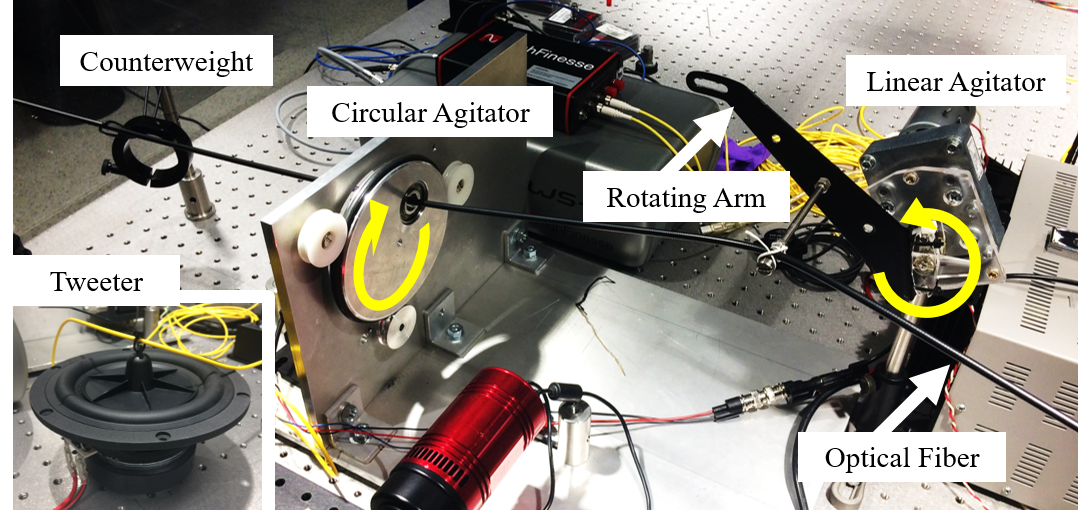
\includegraphics[width=\columnwidth]{images/agitators_labelled.png}
	\caption{Linear and circular agitator used in these modal noise tests. The linear agitator 	rotates along the length of the fiber while the circular agitator rotates perpendicular to it. The counterweight was included to confirm that the fiber would always be taught between the two agitators, preventing it from over-bending or bunching up.}
\label{fig:agitators}
\end{figure} 

All image data was collected with the Fiber Characterization Station (FCS, figure \ref{fig:fcs}), a multipurpose device that is able to simultaneously image the input face, output face (or near field), and output pupil (or far field) of any optical fiber. Specifications for the FCS cameras are listed in table \ref{table:cameras}.

\begin{figure}
\centering
	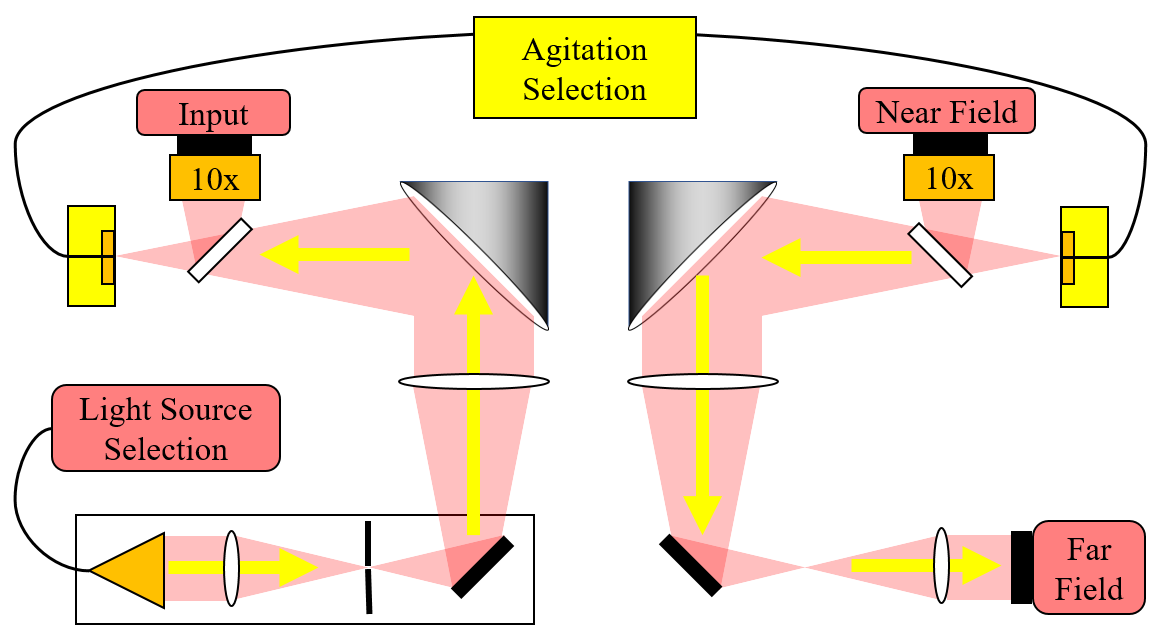
\includegraphics[width=\columnwidth]{images/fcs_schematic.png}
	\caption{Schematic of the Fiber Characterization Station. Light from either a single-mode fiber-fed \SI{652}{\nano\meter} Toptica diode laser or from a selection of Thorlabs mounted LEDs fed by a \SI{100}{\micro\meter} circular fiber is fed into the station in the bottom left. This light is spatially filtered, collimated, and injected into the test fiber. The injection face of the test fiber is imaged at 10x magnification by the input camera to allow for precision alignment. Light propagates through the test fiber and our choice of agitator mixes the modes. Light is then ejected from the test fiber and split between the 10x magnified near field camera and the far field camera.}
\label{fig:fcs}
\end{figure}

\begin{table}
\centering
\caption{Fiber Characterization Station imaging specifications}
	\begin{tabular}{cccccc}
	\hline
	Name & Camera & Pixel Size & Magnification \\
	\hline \hline
	Input & Atik 450 & \SI{3.45}{\micro\meter} & 10 \\
	\hline
	Near Field & Atik 450 & \SI{3.45}{\micro\meter} & 10 \\
	\hline
	Far Field & Atik 383L+ & \SI{5.4}{\micro\meter} & N/A \\
	\hline	
	\end{tabular}
\label{table:cameras}
\end{table}

Modal noise is quantified using the SNR of the near field and far field fiber images calculated as
\begin{equation}
\textrm{SNR}_{nf} = \frac{\textrm{median}(I_{filt})}{\textrm{stdev}(I_0 - I_{filt})}
\end{equation}
and
\begin{equation}
\textrm{SNR}_{ff} = \frac{\textrm{max}(I_{filt})}{\textrm{stdev}(I_0 - I_{filt})}
\end{equation}
respectively where $I_0$, the original raw image, is heavily median filtered to produce $I_{filt}$. The typical SNR could not be used due to intensity varying diffraction effects across the near field fiber image and the Gaussian-shaped far field images. Subtracting $I_{filt}$ from $I_0$ therefore produces a noise pattern that surrounds a flat line profile rather than a curved one. A median filter was used rather than a low-order polynomial or Gaussian fit because these functions were observed to not sufficiently fit the raw fiber images. The ``signal'' was calculated as the median (near field) and maximum (far field) of $I_{filt}$ to prevent dust on the fiber face or optics from skewing this value.

\section{Results}
\label{sec:results}

\subsection{Amplitude and Frequency of Agitation}
\label{subsec:amp_freq}

We used the linear agitator to test the effects of agitation amplitude and frequency of rotation on the SNR. For each parameter, there were two modes of operation: amplitude was set to either \SI{40}{\milli\meter} (low) or \SI{160}{\milli\meter} (high) and frequency was set to either \SI{0.125}{\hertz} (low) or \SI{1.00}{\hertz} (high). Using the \SI{100}{\micro\meter} and \SI{600}{\micro\meter} circular fibers, we took ten images for each of the four possible permutations of these agitation modes and an extra set of ten images using a broadband LED with no agitation.

We set integration times for each image according to the frequency of agitation such that each exposure lasted exactly one rotation of the linear agitator. Therefore, the \SI{1.0}{\hertz} frequency tests had exposures of \SI{1.0}{\second} and the \SI{0.125}{\hertz} frequency tests had exposures of \SI{8.0}{\second}.

We are able to analyze each image individually or any co-added combination of images. Therefore, we can observe the SNR of the modal noise for any amount between one and ten rotations.
 
SNRs for various amplitudes and frequencies of oscillation using the linear agitator with a \SI{200}{\micro\meter} circular fiber are shown in figure [FIGURE NEEDED]. At a fundamental level, these plots show that higher amplitude and higher frequency yield a higher SNR in both the near field and far field. They therefore provide further evidence to support previous intuition about fiber agitation.

\begin{figure}
\centering
	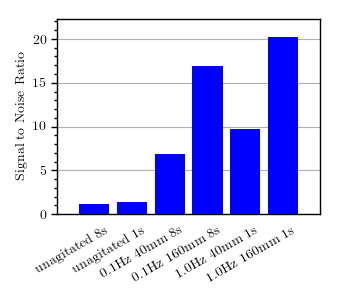
\includegraphics[width=\columnwidth]{images/amp_freq_snr.png}
	\caption{SNR comparison for varying amplitudes and frequencies.}
\label{fig:amp_freq_snr}
\end{figure}

\subsection{Method of Agitation and Fiber Geometry}

We compare the two agitation methods, linear and circular, using a \SI{200}{\micro\meter} circular, \SI{200}{\micro\meter} octagonal, and \SI{100x300}{\micro\meter} rectangular fiber which all have similar cross-sectional area. The two agitators were set to the same amplitude (\SI{40}{\milli\meter}) and frequency (\SI{1.0}{\hertz}).

\begin{figure}
\centering
	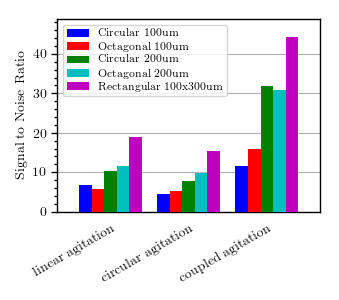
\includegraphics[width=\columnwidth]{images/geom_snr.png}
	\caption{SNR comparison for varying fiber geometries and agitation method}
\label{fig:geom_snr}
\end{figure}

To better understand why coupled agitation is so effective at reducing modal noise, we also analyze the effect of each agitation method over time, as shown in figure \ref{fig:circ_snr_vs_time}. The \SI{200}{\micro\meter} circular fiber shows continued improvement to SNR beyond a single oscillation at \SI{1}{\hertz} at a similar rate to when the fiber is lit by an LED, a broadband source.

\begin{figure}
\centering
	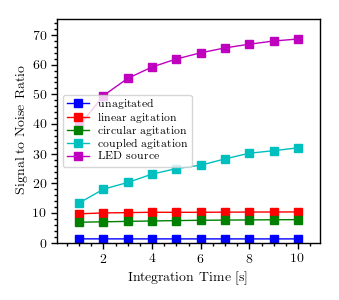
\includegraphics[width=\columnwidth]{images/circ_snr_vs_time.png}
	\caption{SNR for the \SI{200}{\micro\meter} circular fiber using various agitation methods. The SNR is calculated after co-adding \SI{1}{\second} exposure images to the given integration time.}
\label{fig:circ_snr_vs_time}
\end{figure}

\subsection{Fiber Coupling}

Most next-generation RV spectrographs include more than just one fiber when coupling light from the telescope and calibration light sources to the spectrograph. Therefore, we also tested the effects of agitating individual fibers in a multi-fiber assembly where each fiber could have different core diameters and geometries. We tested three distinct cases outlined in table \ref{table:fiber_coupling}.

\begin{table}
\centering
\caption{Fiber assemblies tested for the fiber coupling experiment}
	\begin{tabular}{ccc}
	\hline
	Test & 1st Fiber & 2nd Fiber \\
	\hline \hline
	1 & Circular \SI{200}{\micro\meter} & Circular \SI{200}{\micro\meter} \\
	\hline
	2 & Circular \SI{100}{\micro\meter} & Circular \SI{200}{\micro\meter} \\
	\hline
	3 & Octagonal \SI{200}{\micro\meter} & Circular \SI{200}{\micro\meter} \\
	\hline
	\end{tabular}
\label{table:fiber_coupling}
\end{table}

The results from these tests are shown in figure \ref{fig:coupled_fibers}. The SNR is calculated using the 

\begin{figure}
\centering
	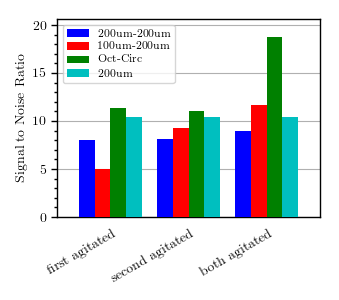
\includegraphics[width=\columnwidth]{images/coupled_fibers.png}
	\caption{SNR for various arrangements of coupled fibers with varying core diameter and cross-sectional shape. The \SI{200}{\micro\meter} bars are a comparison to the single circular fiber agitated with the same amplitude and frequency.}
\label{fig:coupled_fibers}
\end{figure}

\section{Radial Velocity Precision}
\label{sec:rv_precision}

As discussed in section \ref{sec:modal_noise_intro}, optical fiber modal noise is an issue of centroid drift as well as diminished SNR. Therefore, we tested our agitation method over three hundred \SI{1}{\second} exposures to observe how the centroid drifts over time compared to a broadband light source (low modal noise) and a slowly agitated fiber (high modal noise) meant to mimic the slight motions of the telescope throughout a night. The idealized method used in this test included the circular agitator oscillating at \SI{1.1}{\hertz} and the linear agitation set at \SI{120}{\milli\meter} and \SI{1.0}{\hertz}. Keeping the two agitators at slightly different frequencies means that the full range of fiber configurations are reached after about \SI{10}{\second}.

The results for these tests are shown in figure \ref{fig:rv_error} where the RV error is calculated using equation \ref{eq:rv_error}. The dispersion direction for a rectangular fiber is along the short end, meaning that the diameter $D$ is \SI{100}{\micro\meter}. The resolution is assumed to be 150,000, the current goal of EXPRES.

Notice that the rectangular fiber does show RV error due to modal noise in the dispersion direction. This is contrary to the assumption made by \cite{Epworth1978} where spatial filtering is required for modal noise to affect the RV measurement of a spectrograph.

\begin{figure*}
\centering
	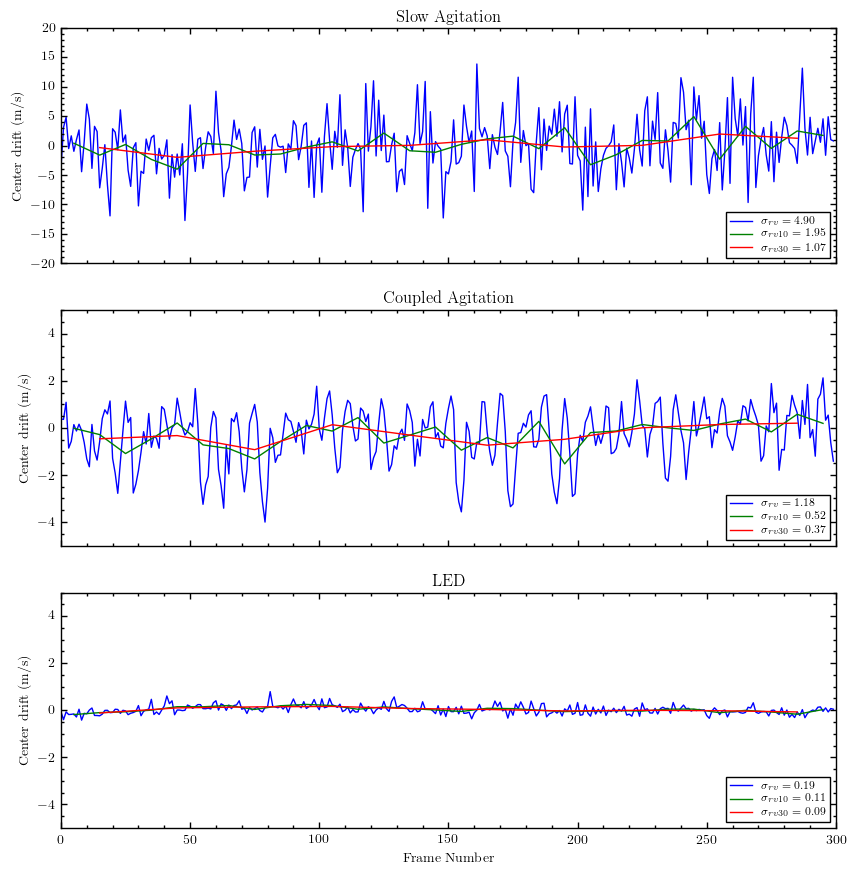
\includegraphics[width=\textwidth]{images/rv_error.png}
	\caption{Centroid drift and resultant RV error for a (a) slowly agitated fiber, (b) coupled agitated fiber, and (c) LED illumination. The red line in each image is the 30-image average of these centroid drifts, effectively yielding the RV error for \SI{30}{second} exposures. Note that the y-scales changes between the slow agitation and coupled agitation plots.}
\label{fig:rv_error}
\end{figure*}

These results indicate that coupled agitation reduces errors induced by a slowly moving telescope by about three-fold and are minimized to about \SI{37}{\centi\meter\per\second}. This error is the RV error per line in the spectrograph, meaning that the total RV error after averaging over 30-40 lines would be less than \SI{10}{\centi\meter\per\second} [INSERT BETTER TOTAL RV ERROR HERE].

Using our prototype agitation setup in our lab, we were not able to reach the stability of continuum illumination (\SI{9}{\centi\meter\per\second}). However, we are confident that increasing the amplitude of circular motion, increasing the frequency of both agitators, and adding a ``tweeter'' element will continue to push this limit even lower.


\section{Discussion and Conclusions}
\label{sec:conclusions}

We have tested a wide swath of agitation parameter space with the goal of further understanding the mechanism behind fiber agitation as a method for modal noise reduction. Our results indicate that large amplitude, relatively high frequency, chaotic coupled harmonic agitation for optical fibers that have large core cross-sectional area and low azimuthal symmetry yielded the highest signal to noise in both the near and far field. We therefore believe that the most important factor when agitating fibers is to place the fiber into as many physical configurations as possible over a single exposure. This motion needs to be continuous, to avoid build-up of a single fiber configuration speckle pattern, and can be done anywhere along the length of the fiber, allowing for large distance from a stabilized spectrograph.

Although most of the tests in this paper look at relatively low frequency agitation (i.e. less than \SI{2}{\hertz}), our conclusions support \cite{Plavchan2013} in that adding a high frequency ``tweeter'' is advantageous to reducing modal noise. During our high-amplitude, high-frequency test from section \ref{subsec:amp_freq}, we observed that the fiber violently shook near the counterweight due to the high torque motion. This test showed significant improvements over high-amplitude with low-frequency, especially at longer exposures, and this appears to be because of this simultaneous high-frequency shaking placing the fiber into extra physical configurations.

These conclusions are highly reminiscent of the idea that hand-agitation is consistently better than any form of mechanical agitation. Human motions are much less deterministic than a motor, meaning that a person hand-agitating the fiber would naturally put it into more physical configurations. Our combined linear/circular agitator with slightly different oscillation frequency mimics this behavior since it will chaotically reach many fiber configurations over a single calibration exposure of approximately [NEED CALIBRATION EXPOSURE TIME] \SI{}{\second}.

The EXPRES fiber assembly will be employing the idealized agitation technique detailed in this paper. We will be combining a \SI{160}{\milli\meter} amplitude circular and linear agitator similar to those seen in figure \ref{fig:agitators}, but with greater stability to support an entire reinforced wrap of cables. The two agitators will oscillate at slightly different frequencies at the maximum speed deemed safe for the fibers. We will also include a large subwoofer speaker attached directly to the cable wrap to add simultaneous high frequency vibrations to the fibers.

\acknowledgments

The Fiber Characterization Station was built with support from the Fund for Astrophysical Research, Inc. Special thanks to Saki Kamon, Kristoffer Acu\~na, and Dominic Eggerman for their data-taking contributions to this project.

\bibliographystyle{aasjournal}  %for bibtex
\bibliography{modal_noise_mitigation} %for bibtex-example

\end{document}